\chapter{Mathematical modelling}

Mathematical models can describe different kinds of dynamic systems, and thus can be used in prediction, analysis abd other tasks. An ideal model in our case, can represent reasonable interactions or effects between immune cells and cytokines and reproduce features and characteristics that were observed in experimental data.

Proposed models for the regeneration process are in the form of non-linear ordinary differential equations (ODE). The only independent variable is post-lesion time $t$, and the equations consists of derivatives of dependent variables (number of cells, mRNA expression of cytokines) with respect to $t$. The equations were mostly an interpretation of the proposed interaction maps, with terms correspond to interaction paths.


\section{Observed data}

Our models were built on the basis of the existing experimental findings from Tsarouchas et al.\cite{ref:Tsarouchas}. The available measurement data included the numbers of three kinds of cells (neutrophil $N$, macrophage $\Phi$ and microglia) and the relative mRNA expression of four kinds of cytokines (il-1$\beta$, tnf-$\alpha$, tgf-$\beta$1a and tgf-$\beta$3). As proposed by Tsarouchas et al., neutrophil and macrophage play important roles in the spinal cord regeneration with il-1$\beta$ and tnf-$\alpha$ being the media. According to this, our initial models focused on the changes of four dependent variables $N$, $\Phi $, $\beta$ (for il-1$\beta$) and $\alpha$ (for tnf-$\alpha$) that are most important and determinative in the regeneration. $N$ and $\Phi$ is of the unit `number of cells', $\beta$ and $\alpha$ was recorded as `relative mRNA expression' (compared to the value at the initla time point i.e. 0 hpl) and considered unitless.

It was noted that the variance of the measured data is relatively high. The summary statistic used for the parameter estimations was mean of measurement data at each time point, assuming that measured data was Gaussian-like distributed. To validate this, the distribution of the measured data points was plotted and examined to see if the mean value can represent the distribution. The result was that at most time points the measurement values are Gaussian-distributed, although some distributions were skewed. One abnormal distribution was observed at time point 120 hpl for macrophage where there are two concentrations. Despite this, mean value could summarise most data and thus was still used as the target observed data. A plot of the mean of the four variables is shown in Figure \ref{fig:obs_data}, which is our target trajectories for the models to fit.

\begin{figure}
    \begin{center}
        \resizebox{1.0\hsize}{!}{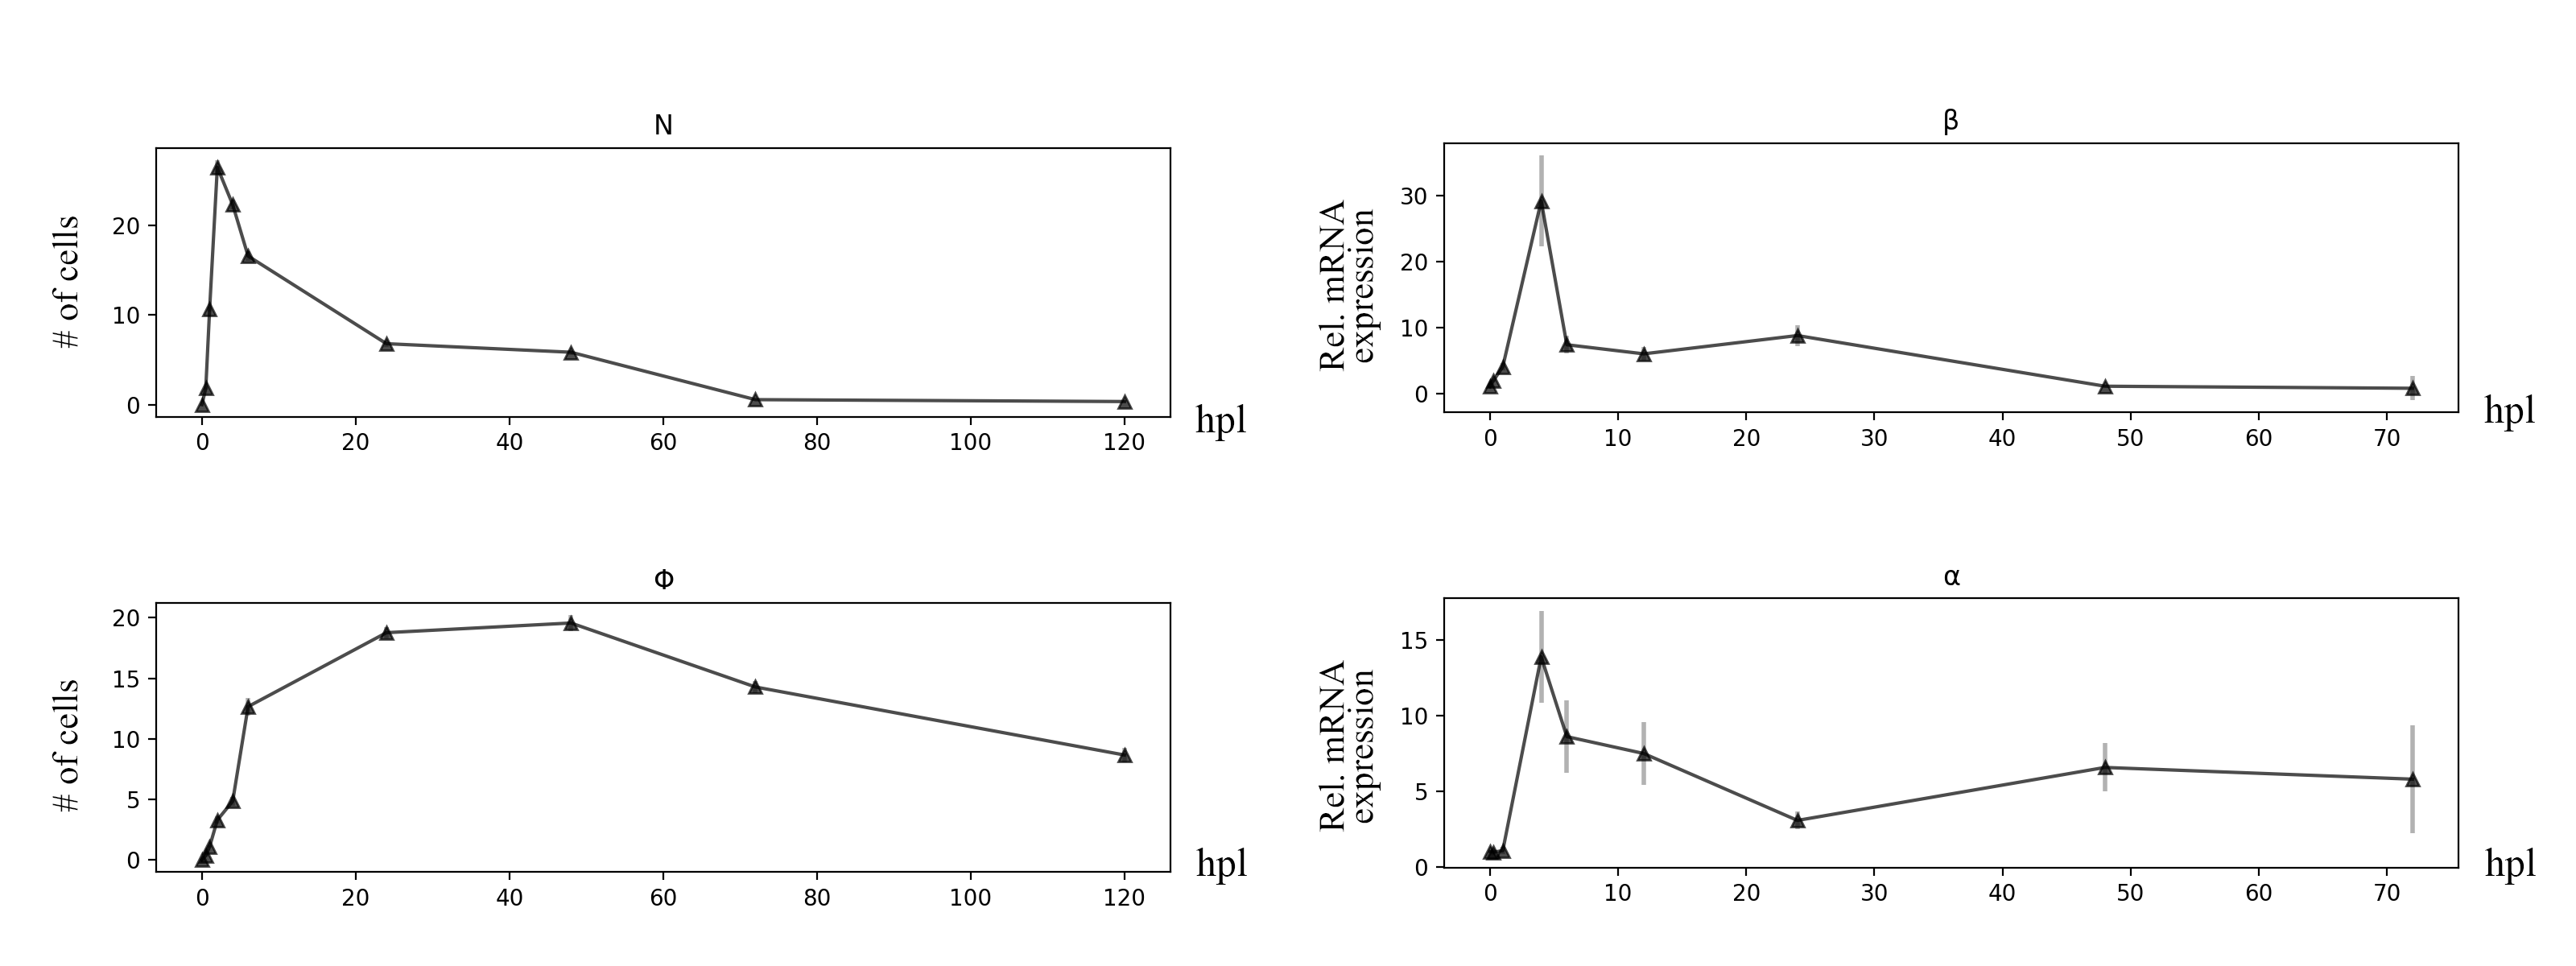
\includegraphics{fig/obs_curve.png}}
    \end{center}

    \caption[Mean of the observed data]%
    {Mean of the observed data for neutrophil ($N$), macrophage ($\Phi$), il-1$\beta$ and tnf-$\alpha$, from experiment results of \cite{ref:Tsarouchas}. Error bars indicate standard error of mean}
    \label{fig:obs_data}

\end{figure}

\section{Hypothesis and models}

5 models in total are proposed according to different hypothesis. At first our tests and implementations of ABC SMC for parameter estimations use only the basic model for developing propose. After the parameter estimation framework is built and tested, more models are proposed, in order to calibrate and adjust the basic model such that it can represent the observed regeneration process better or can be used to test our hypothesis.

All these models assume the involved interactions is within two kinds of cells (neutrophil and macrophage) and two kinds of cytokines (il-1$\beta$ and tnf-$\alpha$) and use the data presented in Figure \ref{fig:obs_data} for the inference task. Interactions or effects from other cells or cytokines is not considered as there might not be corresponding data available.

\subsection{Basic model}

A preliminary model (Eqn. \ref{eq:model1}) was proposed according to \cite{ref:Tsarouchas} and then mainly used to build and test the code of inference framework. An interaction map of the model is shown in Figure \ref{fig:m1}. This model is a simplification a the process described in \cite{ref:Tsarouchas} with some minor interactions ignored. To describe the parameters' units, we denote the unit of $N$ and $\Phi$ i.e. number of cells as `cell', and denote $\beta$ and $\alpha$'s relative mRNA expression as unitless for simplicity. This model included 12 parameters, all of which should be positive real number. A description of these parameters can be found in Table \ref{table:m1}.

\begin{figure}
    \begin{center}
        \resizebox{0.4\hsize}{!}{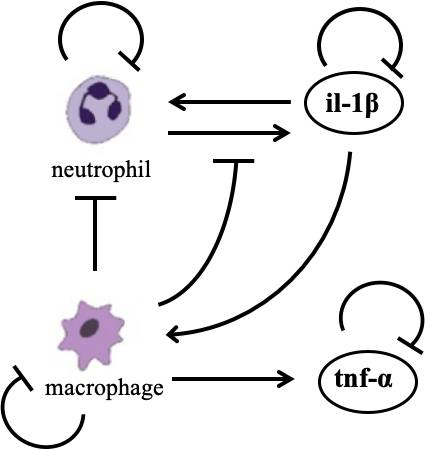
\includegraphics{fig/model1.png}}
    \end{center}

    \caption[Interactions modelled in the basic model]%
    {Interactions modelled in the basic model (model 1) based on Tsarouchas et al.\cite{ref:Tsarouchas}. Lines ended with arrow represent promoting effect, lines ended with T-connectors represent inhibition}
    \label{fig:m1}

\end{figure}

It was assumed that there were negative feedbacks the cells and cytokines, i.e. overcrowding inhibits the increasing rates. 

MORE DESCRIBE.

\begin{align}
    \label{eq:model1}
    \begin{split}
        &\frac{\mathrm{d} N}{\mathrm{d} t}=\lambda_N+\kappa_{N\beta}\beta-\mu_NN-\nu_{N\Phi}N\Phi\\
        &\frac{\mathrm{d} \Phi}{\mathrm{d} t}=\lambda_\Phi+\kappa_{\Phi\beta}\beta-\mu_\Phi\Phi\\
        &\frac{\mathrm{d} \beta}{\mathrm{d} t}=\frac{s_{\beta N}N}{1+i_{\beta\Phi}\Phi}-\mu_\beta\beta\\
        &\frac{\mathrm{d} \alpha}{\mathrm{d} t}=s_{\alpha\Phi}\Phi-\mu_\alpha\alpha
    \end{split}
\end{align}

\begin{table}[h!]
    \centering
    \begin{tabular}{|c c c|}
        \hline
        Parameter            & Definition                                       & Units                    \\ [0.5ex]
        \hline\hline
        $\lambda_N$          & Self-increase rate of neutrophil                 & $cell/h$                 \\
        $\kappa_{N\beta}$    & Promoting effect coefficient by il-1$\beta$      & $cell/(unit\cdotp h)$    \\
        $\mu_N$              & Coefficient of negative feedback of $N$          & $h^{-1}$                 \\
        $\nu_{N\Phi}$        & Coefficient of inhibition of both $N$ and $\Phi$ & $cell^{-1}\cdotp h^{-1}$ \\
        \hline
        $\lambda_\Phi$       & Self-increase rate of macrophage                 & $cell/h$                 \\
        $\kappa_{\Phi\beta}$ & Promoting effect coefficient by il-1$\beta$      & $cell/(unit\cdotp h)$    \\
        $\mu_\Phi$           & Coefficient of negative feedback of $\Phi$       & $h^{-1}$                 \\
        \hline
        $s_{\beta N}$        & Production rate from $N$                         & $unit/(cell\cdotp h)$    \\
        $i_{\beta\Phi}$      & Coefficient of inhibition to the production      & $cell^{-1}$              \\
        $\mu_\beta$          & Coefficient of negative feedback of $\beta$      & $h^{-1}$                 \\
        \hline
        $s_{\alpha\Phi}$     & Production rate from $\Phi$                      & $unit/(cell\cdotp h)$    \\
        $\mu_\alpha$         & Coefficient of negative feedback of $\alpha$     & $h^{-1}$                 \\
        \hline
    \end{tabular}
    \caption{Parameters introduced in the basic model (model 1) [REMOVE unit]}
    \label{table:m1}
\end{table}

\subsection{Alternative models}

\paragraph{Model 2 and model 3}

As the observed data indicate, this dynamic system has a steady state where the  inflammation is resolved and immune cells should not be present at the injury site. Regarding this, the self-increase parameter $\lambda$ cannot be constant, thus a exponentially decaying $\lambda$ term is introduced and model 2 is proposed. (Eqn. \ref{eq:model2}). Also, the inhibition of il-1$\beta$ production, i.e. term $i_{\beta\Phi}\Phi$ is considered to be ignored for a more simple model, in which case the relative expression of il-1$\beta$ is only affected by the number of neutrophil and the negative feedback from itself. This case corresponds to model 3, written as Eqn. \ref{eq:model3}.

Model 2 and model 3 introduce one extra parameter $a$, which is a coefficient in the exponentially decaying $\lambda$, determining the decay speed, with the unit $h^{-1}$.

\begin{align}
    \label{eq:model2}
    \begin{split}
        &\frac{\mathrm{d} N}{\mathrm{d} t}=\lambda_Ne^{-at}+\kappa_{N\beta}\beta-\mu_NN-\nu_{N\Phi}N\Phi\\
        &\frac{\mathrm{d} \Phi}{\mathrm{d} t}=\kappa_{\Phi\beta}\beta-\mu_\Phi\Phi\\
        &\frac{\mathrm{d} \beta}{\mathrm{d} t}=\frac{s_{\beta N}N}{1+i_{\beta\Phi}\Phi}-\mu_\beta\beta\\
        &\frac{\mathrm{d} \alpha}{\mathrm{d} t}=s_{\alpha\Phi}\Phi-\mu_\alpha\alpha
    \end{split}
\end{align}

\begin{align}
    \label{eq:model3}
    \begin{split}
        &\frac{\mathrm{d} N}{\mathrm{d} t}=\lambda_Ne^{-at}+\kappa_{N\beta}\beta-\mu_NN-\nu_{N\Phi}N\Phi\\
        &\frac{\mathrm{d} \Phi}{\mathrm{d} t}=\kappa_{\Phi\beta}\beta-\mu_\Phi\Phi\\
        &\frac{\mathrm{d} \beta}{\mathrm{d} t}=s_{\beta N}N-\mu_\beta\beta\\
        &\frac{\mathrm{d} \alpha}{\mathrm{d} t}=s_{\alpha\Phi}\Phi-\mu_\alpha\alpha
    \end{split}
\end{align}

Model 3 can be regarded as a simplification of model 2, as it can be treated as model 2 with parameter $i_{\beta\Phi}=0$. Among the proposed three models, model 1 is a naive one that was proposed at very first time and used as an ODE `template' to build and test parameter inference framework. As the implementation was successful, model 2 and 3 was proposed as we were trying to calibrate some terms and find a better model. After fitting, model 2 is supposed to be better than model 1 as it corrects the problem that appears at the final time points (which relate to the steady state). Model 3 makes a small simplification on model 2 and is theoretically less `general' than model 2.

\paragraph{Model 4 and model 5}

After the first model selection experiment, it was found that some significant features presented in the observed data were not recovered by any of the existing model. To resolve this, attempts were tried to introduce more interactions within the dynamic system considering the biological and  mathematical context. Extra promoting effect to the expression of tnf-$\alpha$ was considered, by either adding a phenomenological term (which means the same effect as directly promoting but the underlying mechanism is unclean) or adding a term that represents a promoting effect to the production process of tnf-$\alpha$, namely model 4 (Eqn. \ref{eq:model4}) and model 5 (Eqn. \ref{eq:model5}).

\begin{align}
    \label{eq:model4}
    \begin{split}
        &\frac{\mathrm{d} N}{\mathrm{d} t}=\lambda_Ne^{-at}+\kappa_{N\beta}\beta-\mu_NN-\nu_{N\Phi}N\Phi\\
        &\frac{\mathrm{d} \Phi}{\mathrm{d} t}=\kappa_{\Phi\beta}\beta-\mu_\Phi\Phi\\
        &\frac{\mathrm{d} \beta}{\mathrm{d} t}=s_{\beta N}N-\mu_\beta\beta\\
        &\frac{\mathrm{d} \alpha}{\mathrm{d} t}=s_{\alpha\Phi}\Phi-\mu_\alpha\alpha+d_{\beta\alpha}\beta
    \end{split}
\end{align}

\begin{align}
    \label{eq:model5}
    \begin{split}
        &\frac{\mathrm{d} N}{\mathrm{d} t}=\lambda_Ne^{-at}+\kappa_{N\beta}\beta-\mu_NN-\nu_{N\Phi}N\Phi\\
        &\frac{\mathrm{d} \Phi}{\mathrm{d} t}=\kappa_{\Phi\beta}\beta-\mu_\Phi\Phi\\
        &\frac{\mathrm{d} \beta}{\mathrm{d} t}=s_{\beta N}N-\mu_\beta\beta\\
        &\frac{\mathrm{d} \alpha}{\mathrm{d} t}=(s_{\alpha\Phi}+f_{\beta\alpha}\beta)\Phi-\mu_\alpha\alpha
    \end{split}
\end{align}

\begin{table}[h!]
    \centering
    \begin{tabular}{|c c c|}
        \hline
        Parameter         & Definition                                                     & Units                    \\ [0.5ex]
        \hline\hline
        $d_{\beta\alpha}$ & Coefficient of promoting effect from $\beta$                   & $h^{-1}$                 \\
        \hline
        $f_{\beta\alpha}$ & Coefficient of promoting the production of $\alpha$ by $\beta$ & $cell^{-1}\cdotp h^{-1}$ \\
        \hline
    \end{tabular}
    \caption{Parameters introduced in model 4 and 5}
    \label{table:m45}
\end{table}



\subsection{Model evaluation and comparison}

[general topics on evaluating a model]

[bayes factor for model selection]

\subsection{Limitations}

[hypothesis]

[available data]

[model misspecification]

% \begin{figure}

% \begin{center}
% \resizebox{0.30\hsize}{!}{
\includegraphics{logos/crest_bw}}
% \end{center}

% \caption{The University Crest}
% \label{fig:eucrest}

% \end{figure}


% see the man page for dvips for details of the special command which is
% much more powerful than is shown here. It allows offsets in the
% horizontal and vertical and scaling in x and y.

% choosing suitable values for offset and scale can be a tiring matter
% of trial and error.

% note that labels do not need to include a description of the object
% they are labelling but it can be helpful, eg \label{fig:figurename}.

% You can use a label on a figure to refer to it later. The university
% crest is in \ref{fig:eucrest}. Note that you should not use phrases like
% ``the figure above'' or ``the following figure'' since Latex may move
% the figure relative to the text if it cannot be fitted onto the current page.






